%Results
\section{Descriptive statistics}
Before the experiment, the seeds were weighted in groups of ten, to see if there was a baseline difference between certain genotypes. Table \ref{tab:germination_percentage}, in the previous section, displays the measured weights.
After the completion of the experiment, the outliers were identified, and each plant was attributed a specific weight, following the protocol described in the material and methods section. Those weights were used to compute the weighted mean and weighted standard deviation of the fresh and dry weight of the root system and the leaf system for each plant. Even though we have four variables in our analysis, it is important to notice that there is a high correlation between the variables (see Table \ref{tab:var_correlation}) and that in a future trial, the analysis of other less-correlated variables (non-measured here) could be interesting.\\

\begin{table}[ht]
\rowcolors{2}{gray!25}{white}
\centering
 \caption{Correlation matrix of the four variables.}
\begin{tabular}{lrrrr}
  \hline
 & DRY\_LS & DRY\_RS & FRESH\_RS & FRESH\_LS \\ 
  \hline
DRY\_LS & 1.00 & 0.70 & 0.84 & 0.93 \\ 
  DRY\_RS & 0.70 & 1.00 & 0.76 & 0.68 \\ 
  FRESH\_RS & 0.84 & 0.76 & 1.00 & 0.93 \\ 
  FRESH\_LS & 0.93 & 0.68 & 0.93 & 1.00 \\ 
   \hline
\end{tabular}
\label{tab:var_correlation}
\end{table}

Because of germination problems on the platform and inside the germination chamber, not all genotypes were similarly represented in the experiment. Table \ref{tab:updated_germ_rates} presents the effective germination rates for each genotype, i.e. the number of seed actually kept for the spatial analysis over the number of seeds placed on the platform. This table is interesting because germination rate is a genotypic feature. Since the genotypes are sorted by their effective germination rate, we see clear discrepancies between genotypes, indicating that some may not be well suited to aeroponic growth. Only 6 genotypes have a germination rate lower than 50\% (below the dashed line on Table \ref{tab:updated_germ_rates}), even though more than 15 seeds where placed on the platform. Thus, we expect to see a lower yield in all variables for these genotypes. However, the results presented in Figure \ref{fig:dotplot_all_variables} do not show the same order of genotypes, suggesting that the germination potential and the growth are not influenced in the same way by the genotypic features and by the environment.\\

To check those assumptions, we created boxplots ordered by descending mean value for tank A, presented in Figure \ref{fig:dotplot_all_variables}. The numerical values of these results are presented in Table \ref{tab:summary_table_all_variables}, in Appendix \ref{appendix:mean_std_table}.
The mean value for tank A is almost always higher than for tank B expect for some genotypes (21, 30, 22 and 12 on Figure a), letting us believe that those genotypes might be more suited to a still growing environment. Apart from those, there is a clear difference in yield between the two tanks, but it is more pronounced for the fresh weights. Overall the values in tank B seem to have less variations than in tank A, this might be an effect of the moving versus still conditions. Even though the order of the genotypes is not the same for all variables, some genotypes (e.g. 16, 4, 6 and 29 on all Figures) always show a high mean value.
This implies that the tank and genotypes effects might be significant. In order to further test that, an analysis of the mean differences can be useful. 


\begin{table}[hbtp]
  \rowcolors{2}{gray!25}{white}
\centering
\caption[Effective germination rates]{Effective on-platform germination rates (GR) with the number of seeds kept for data analysis (NS kept) and the number 
of seeds actually placed on the platform (NS placed) for each genotype. The dotted line represents the 50\% germination rate limit.} 
\begin{minipage}{0.45\textwidth}
\begin{tabular}{lrrr}
  \toprule
Genotype & NS placed & NS kept & GR \\ 
  \midrule
25 & 29 & 27 & 93.1 \\ 
  23 & 22 & 20 & 90.9 \\ 
  16 & 27 & 23 & 85.2 \\ 
  18 & 26 & 22 & 84.6 \\ 
  3 & 29 & 24 & 82.8 \\ 
  17 & 27 & 21 & 77.8 \\ 
  19 & 30 & 23 & 76.7 \\ 
  1 & 24 & 18 & 75.0 \\ 
  12 & 28 & 21 & 75.0 \\ 
  14 & 26 & 19 & 73.1 \\ 
  28 & 26 & 19 & 73.1 \\ 
  9 & 29 & 20 & 69.0 \\ 
  6 & 29 & 19 & 65.5 \\ 
  7 & 29 & 19 & 65.5 \\ 
  4 & 23 & 15 & 65.2 \\
  \vdots & \vdots & \vdots & \vdots \\
  \bottomrule
 \end{tabular}
 
\end{minipage} \hfill
\begin{minipage}{0.45\textwidth}
 \begin{tabular}{lrrr}
   \toprule
Genotype & NS placed & NS kept & GR \\ 
  \midrule
    \vdots & \vdots & \vdots & \vdots \\
  27 & 29 & 18 & 62.1 \\ 
  21 & 26 & 16 & 61.5 \\ 
  5 & 30 & 18 & 60.0 \\ 
  24 & 30 & 18 & 60.0 \\ 
  10 & 29 & 17 & 58.6 \\ 
  20 & 26 & 15 & 57.7 \\ 
  22 & 18 & 10 & 55.6 \\ 
  29 & 28 & 15 & 53.6 \\ 
  13 & 27 & 14 & 51.9 \\\hdashline 
  15 & 18 & 9 & 50.0 \\ 
  2 & 26 & 12 & 46.2 \\ 
  11 & 19 & 8 & 42.1 \\ 
  26 & 29 & 12 & 41.4 \\ 
  8 & 21 & 8 & 38.1 \\ 
  30 & 23 & 3 & 13.0 \\ 
   \bottomrule
\end{tabular}

 \end{minipage}
\label{tab:updated_germ_rates}
\end{table}


\begin{figure}
\centering
	\begin{subfigure}[t]{\textwidth}
	\label{fig:desc_stat_DRY_LS}
		\centering
		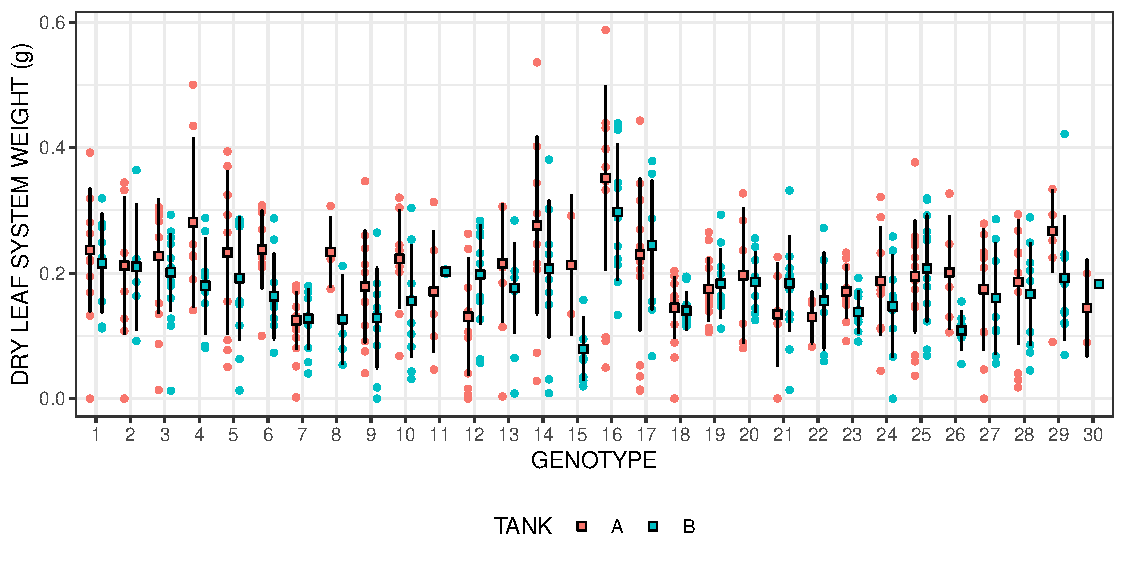
\includegraphics[width = \textwidth]{../../Figures/DRY_LS_summary_plot.pdf}
		\caption{Dry leaf weight ($DRY\_LS$)}
			\end{subfigure}

	\begin{subfigure}[t]{\textwidth}
		\centering
		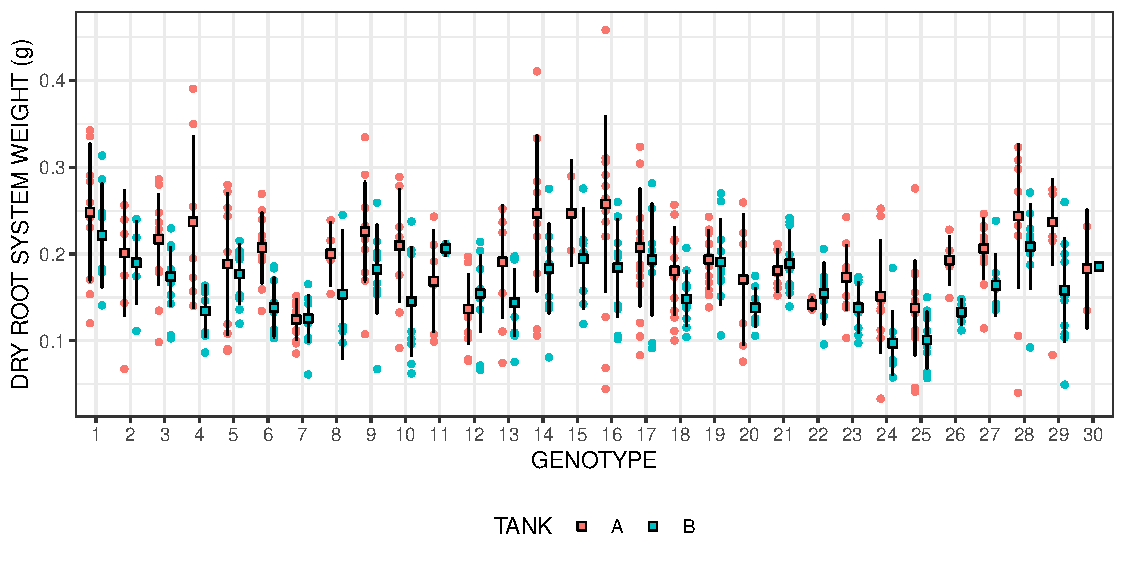
\includegraphics[width = \textwidth]{../../Figures/DRY_RS_summary_plot.pdf}
		\caption{Dry root weight ($DRY\_RS$)}
	\end{subfigure}
	\caption[Boxplot of the mean weight and associated standard deviation]{Boxplot displaying mean weight (\protect\emptysquare) and associated standard deviation (\protect\blackline), grouped by tanks and ordered by descending mean value for tank A.}
\end{figure}
\begin{figure}\ContinuedFloat
	\captionsetup[figure]{list=no}
	\begin{subfigure}[t]{\textwidth}
		\centering
		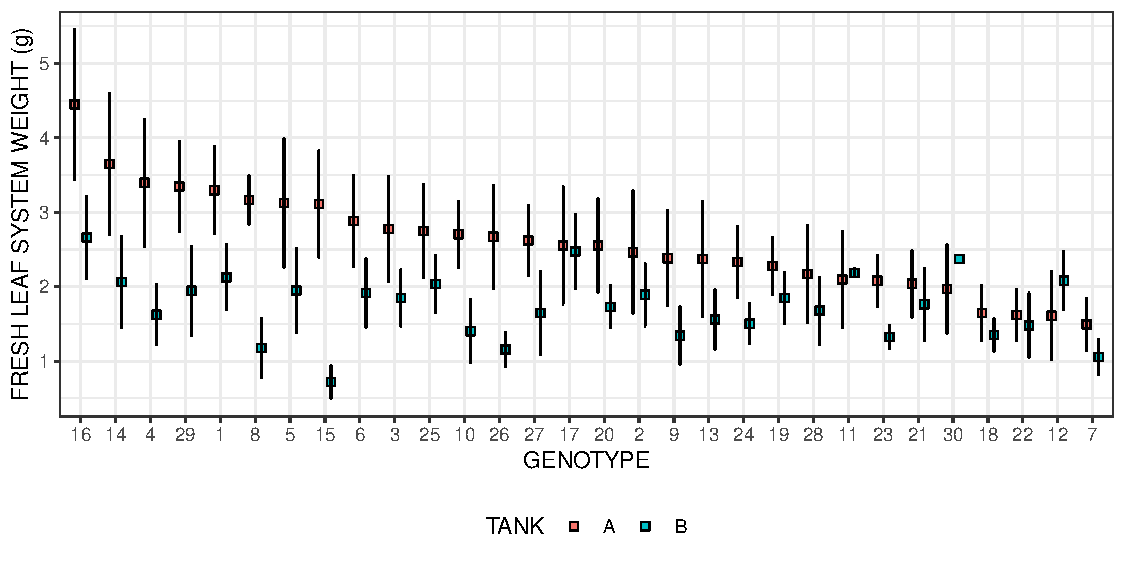
\includegraphics[width = \textwidth]{../../Figures/FRESH_LS_summary_plot.pdf}
		\caption{Fresh leaf weight ($FRESH\_LS$)}
	\end{subfigure}

	\begin{subfigure}[t]{\textwidth}
		\centering
		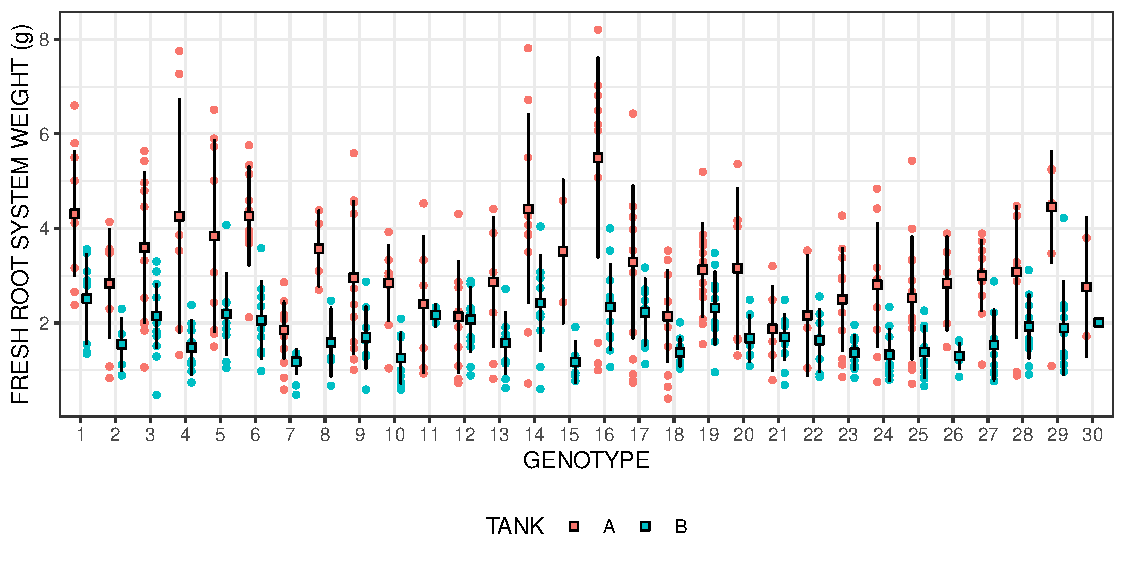
\includegraphics[width = \textwidth]{../../Figures/FRESH_RS_summary_plot.pdf}
		\caption{Fresh root weight ($FRESH\_RS$)}
	\end{subfigure}
	\caption[Boxplot of the mean weight and associated standard deviation]{Boxplot displaying mean weight (\protect\emptysquare) and associated standard deviation (\protect\blackline), grouped by tanks and order by descending mean value for tank A.}
	\label{fig:dotplot_all_variables}
\end{figure}

\section{SpATS analysis}
For the SpATS model, we analysed the four weight variables using the following model:
\begin{equation}
	\mathbf{y} =\mathbf{X} \boldsymbol{\beta}_{T} +\mathbf{X}_{s} \boldsymbol{\beta}_{s}+\mathbf{Z}_{s} \mathbf{s}+\mathbf{Z}_{u} \mathbf{u}
	+ \mathbf{Z}_{v} \mathbf{v} + \mathbf{Z}_{g} \mathbf{g}+ \mathbf{e} \text{,}
\end{equation}
where:
\begin{itemize}
	\item $\mathbf{X} \beta_{T}$ is the fixed term for the tanks,
	\item $\mathbf{X}_{s} \boldsymbol{\beta}_{s}+\mathbf{Z}_{s} \mathbf{s}$ is the mixed model representation of the bivariate smooth surface $f(\mathbf{u},\mathbf{v})$,
	\item $\mathbf{Z}_{u} \mathbf{u}$ is the random effect of the rows,
	\item $\mathbf{Z}_{v} \mathbf{v}$ is the random effect for the columns,
	\item $\mathbf{Z}_{g} \mathbf{g}$ is the random effect for the genotypes, and 
	\item $\mathbf{e}$ is the residual error.
\end{itemize}

The analysis of the results is split in 2 parts:
\begin{enumerate}
	\item A visual analysis of the fitted values and the residuals compared to the raw data; to see if the 
	spatial patterns have been accounted for by the spatial model.
	\item An analysis of the individual contribution of each term of the bivariate smooth surface $f(\mathbf{u},\mathbf{v})$.
	%\item A comparison of the variance of all the random term to see which one were the most influential in the model.
\end{enumerate}
The analysis of the estimated coefficient for the genotypes and for the tanks is presented in a following section, with the estimates of the BSS model.

\subsection{Visual analysis}
The raw data, the fitted data and the spatial model residuals are presented, for all variables, in Figure \ref{fig:spats_model_results}. The raw data shows us that the difference between tanks is less pronounced for the dry weights than for the fresh weights. However, this difference is well represented in the fitted data, where tank B (on the right in each picture) consistently display lower weight values. A strip effect is also noticeable for tank B, where the last strips have lower values than the first ones. This might be an effect of the still growing environment, since this effect is not present in tank A, which was constantly moving. No clear pattern emerges from the residuals, expect the fact that tank A seems to have more single data point with lower values the were not picked up by the spatial surface. Since those points are different than their local neighbours, it is possible that the model had trouble accounting for these local heterogeneities. A analysis of the residuals distribution revealed no violation to the normality assumption.\\

Furthermore, a comparison of the scales of the fitted values and the raw data on Figure \ref{fig:spats_model_results} shows us that the smooth surface could not account for the extreme values present in the raw data. For example the range of the weight values for FRESH\_RS is 8, whereas it only goes to 5 for the fitted surface. However, the scale of the residuals is lower than the one of the fitted values, indicating that the smooth surface accounts for a good amount of the spatial variation.

\begin{figure}
	\begin{subfigure}[t]{\textwidth}
		\centering
		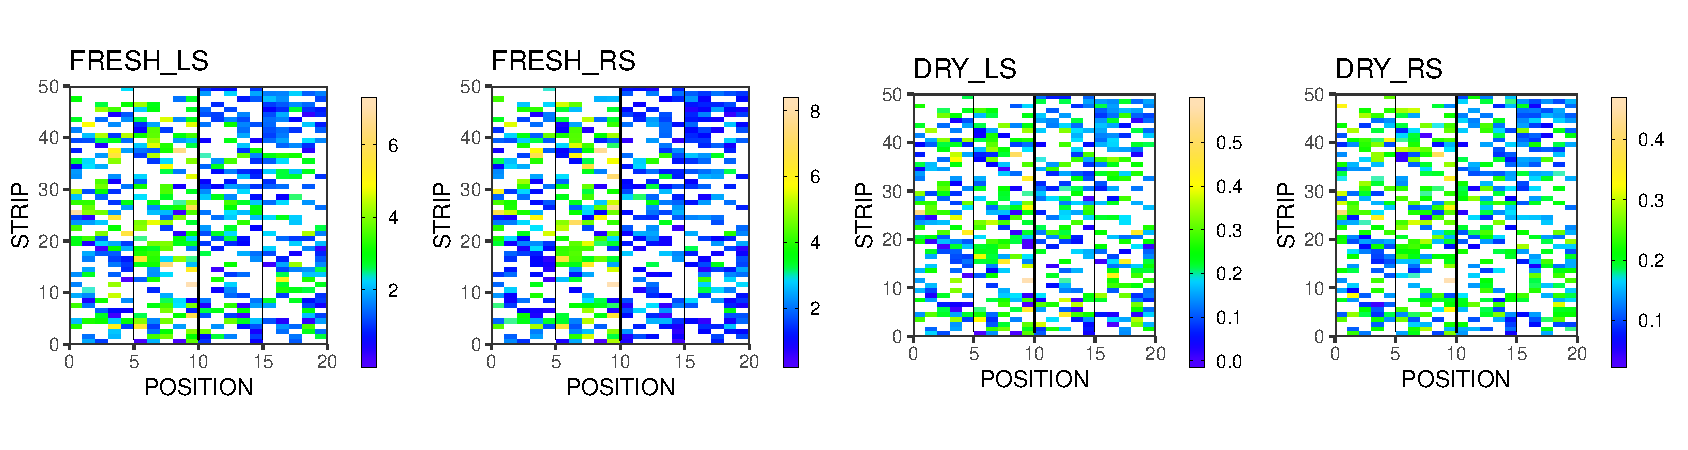
\includegraphics[width = \textwidth]{../../Figures/SPATS_rawData_plot.pdf}
		\caption{Raw data}
	\end{subfigure}
	
	\begin{subfigure}[t]{\textwidth}
		\centering
		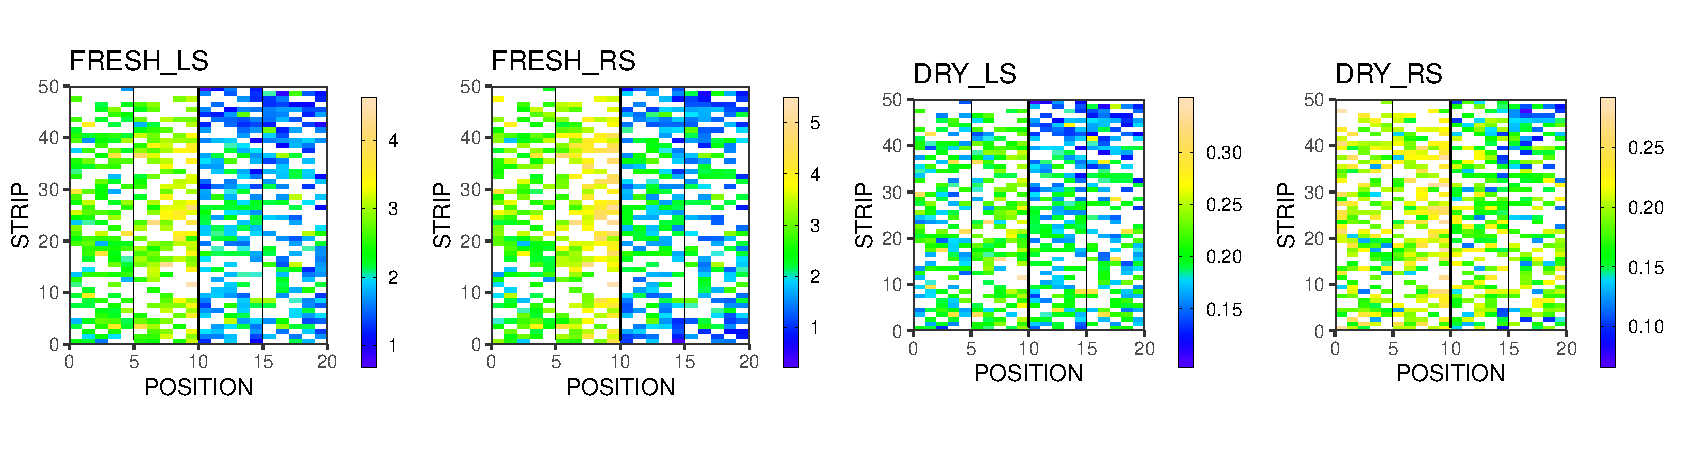
\includegraphics[width = \textwidth]{../../Figures/SPATS_Fitted_plot.pdf}
		\caption{Fitted spatial trend}
	\end{subfigure}
	
	\begin{subfigure}[t]{\textwidth}
		\centering
		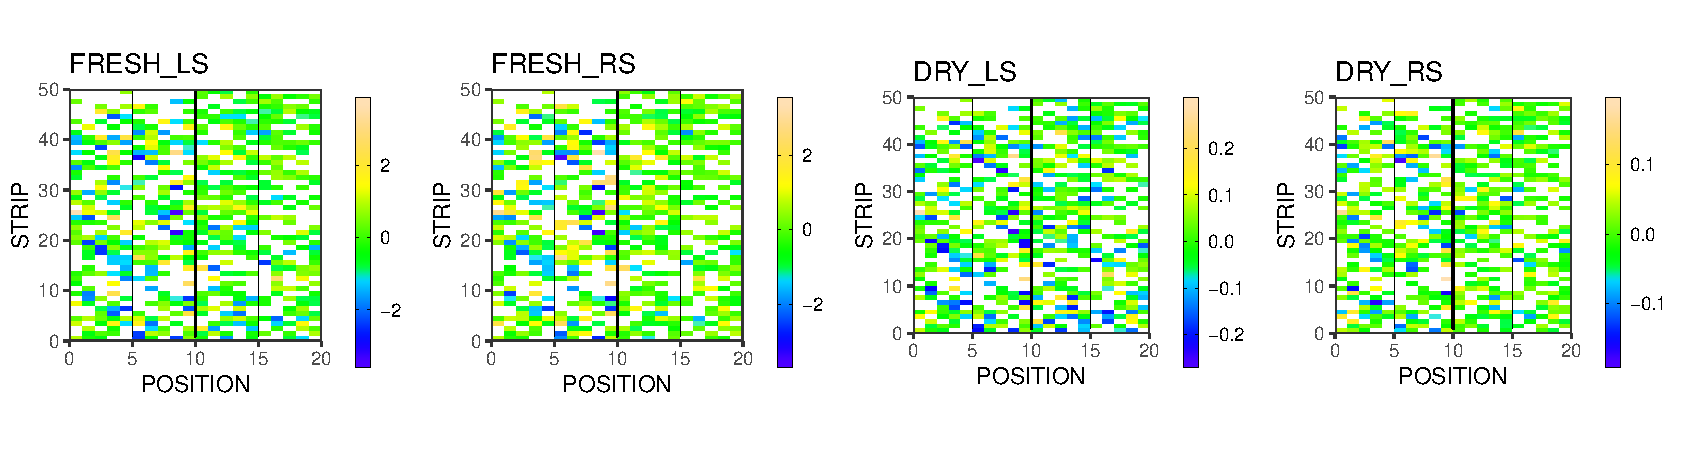
\includegraphics[width = \textwidth]{../../Figures/SPATS_residuals_plot.pdf}
		\caption{Residuals' spatial plot}
	\end{subfigure}
	\caption{Raw data, fitted spatial trend and residuals' plot for each variable.}
	\label{fig:spats_model_results}
\end{figure}

\subsection{Smooth surface terms analysis}
The smooth part of the smooth bivariate surface can be decomposed in the following terms:
\begin{equation}
	f_{u}(\boldsymbol{u})+f_{v}(\boldsymbol{v})+\boldsymbol{u} \odot h_{v}(\boldsymbol{v})+\boldsymbol{v} \odot h_{u}(\boldsymbol{u})+f_{u, v}(\boldsymbol{u}, \boldsymbol{v}) \text{,}
\end{equation}
that are linear terms, linear-by smooth and smooth-by-smooth interaction terms (see section \ref{sec:spats_model} for more details). As explained in the previous chapter, the contribution of each term to the whole surface can be assessed using the effective dimension of each component. Table \ref{tab:spats_dimensions} presents the contribution of each term for each variable as the percentage of the total effective dimension of the smooth surface.\\

For the fresh weights, the smooth-by-smooth interaction ($f_{u, v}(\boldsymbol{u}, \boldsymbol{v})$) represents almost 70\% of the total surface variation. This emphasizes the complexity of the spatial patterns. The smooth-by-linear along the strips interaction ($\boldsymbol{u} \odot h_{v}(\boldsymbol{v})$) and the smooth along the strips ($f_{u}(\mathbf{u})$ ) terms account for the rest of the variation. This confirms that there is more variation along the strips than along the positions.\\

For the dry weights, the variation is shared among all the terms except for smooth along the position that accounts for nothing. This means that there were less heterogeneous spatial variation and more smooth gradients than for the fresh-weights. Indeed, if we look back at the fitted residuals on Figure \ref{fig:spats_model_results}, we see clearly that there is a gradient among the strips and the positions, instead of random patches of high yield.\\

The total effective dimension is also presented because it is an indicator of the overall complexity of the spatial patterns that the smooth surface models. Since the total is lower for the dry weights, it confirms again that the spatial variability was less complex for those variables. As explained in the previous chapter, the effective dimension of a parameter, is proportional to its variance. Therefore, a table presenting the variance of all the random components of the models is presented in Appendix \ref{appendix:tab_spats_variances}

% Table generated by Excel2LaTeX from sheet 'Sheet2'
\begin{table}[htbp]
  \rowcolors{2}{gray!25}{white}
  \centering
  \caption[Effective dimensions of the SpATS model]{Contribution of each component of the spatial smooth surface as a percentage 
  of the total effective dimension of the surface. Here $\boldsymbol{v}$ represents the columns, i.e. the position on the strip; 
  and $\boldsymbol{u}$ represents the rows, i.e. the strip itself.}
	\begin{threeparttable}  
  	    \begin{tabular}{lrrrr}
	    \toprule
	    \begin{tabular}[b]{@{}l@{}}Model \\ \rowcolor{white} components\end{tabular} & \multicolumn{1}{l}{FRESH\_LS} & 
	    \multicolumn{1}{l}{FRESH\_RS} & \multicolumn{1}{l}{DRY\_LS} & \multicolumn{1}{l}{DRY\_RS} \\
	    \midrule
	    $f_{v}(\mathbf{v})$ 								& 0\tnote{$\dagger$} & 0 & 0 & 0  \\
	    $f_{u}(\mathbf{u})$ 								& 8.73 & 14,10 & 17,26 & 17,26 \\
	    $\boldsymbol{u} \odot h_{v}(\boldsymbol{v})$ 		& 19,95 & 16,40 & 24,77 & 24,77 \\
	    $\boldsymbol{v} \odot h_{u}(\boldsymbol{u})$ 		& 2,56 & 0 & 18,36 & 18,36 \\
	    $f_{u, v}(\boldsymbol{u}, \boldsymbol{v})$ 			& 68,76 & 69,5 & 39,62 & 39,62 \\
	    \midrule
	    Total 												& 9,21 (100\%) & 16,15 (100\%) & 5,93 (100\%)& 4,91 (100\%) \\
	    \bottomrule
	    \end{tabular}%
	    \begin{tablenotes}
	    	\item[$\dagger$] All values inferior to 0.0001\% were marked as 0 in the table.
	  	\end{tablenotes}
	\end{threeparttable}
  \label{tab:spats_dimensions}%
\end{table}%


\section{Standard spatial model analysis}
For the standard spatial model analysis,we fitted a baseline model, only considering a fixed effect for the tanks and a random effect for the genotypes and spatially independent residuals:
\begin{equation}
	\mathbf{y} =\mathbf{X} \boldsymbol{\beta}_{T} + \mathbf{Z}_{g} \mathbf{g}+ \mathbf{e} \text{.}
\end{equation}
The model was then augmented separately for each variable, by adding linear regression terms on the rows and columns and one of the following covariance structure:
\begin{itemize}
\item $AR(1)$ process along the rows or columns
\item $AR(1) \times AR(1)$ process
\item $LV$ process along the rows or columns
\item Superimposed row and column structure $LV + LV$
\item Separable process along the rows or columns $LV\otimes J$
\item Separable process along the rows and columns $LV \times LV$
\end{itemize}
At each step, the AIC  was computed and used to select the best model (a lower value is preferred). Table \ref{tab:selected_BSS_models} gives the structure of the final selected model for each variable.\\

\begin{table}[htbp]
  \rowcolors{2}{gray!25}{white}
  \centering
  \caption[Selected BSS models]{Best standard spatial (BSS) model selected for each of the four variables. All the models 
  contain an intercept and a fixed effect for the tank and a random effect for the genotypes. $P$ represents a random effect for the positions (columns), $S$ a random effect for the strips (rows) and $n$ represent the spatially independent residuals.}
    \begin{tabular}{ll}
    \toprule
    Variable & \multicolumn{1}{l}{BSS} \\
    \midrule
    FRESH\_LS & $ S + AR(1) \times AR(1)$  \\
    FRESH\_RS &  $ S + AR(1) \times AR(1)$ \\
    DRY\_LS & $S + P + LV\times LV$ \\
    DRY\_RS &  $S + P + LV+LV$\\
    \bottomrule
    \end{tabular}%
\label{tab:selected_BSS_models}
\end{table}%

First, we see that, for the fresh weights, the models only contains a random effect on the strips (rows) and not the positions (columns). This is similar to the interpretation of the effective dimensions of the SpATS model from Table \ref{tab:spats_dimensions}, that highlighted the strong strip effect and the almost non-existing position effect for the fresh weights. However, all models used a strips-by-positions covariance structure, illustrating the fact that the spatial trends display complex patterns that cannot be accounted for by a one dimensional process only \\

Then, we see that the fresh weights were best represented by an auto-regressive process whereas the dry weights needed a linear covariance structure. \textcite{piepho_linear_2010} explain that both structures give similar results with large auto-correlation ($\rho$) values, which is the case here (see table \ref{tab:BSS_variance_values}) but that the LV structure is more robust to convergence issues. Since we encountered some convergence problems when fitting the $AR(1)$ structure on the dry weight models, it might explain the better AIC value of the $LV$ models.

Finally, both dry weight models use a linear covariance structure but DRY\_LS uses the superimposed structures whereas DRY\_LS uses the separable model. The only difference between those models is the way they model the pairwise variances for plots on different strips (rows) and different positions (columns), but overall they yield similar results in most cases \parencite{piepho_linear_2010}.\\

Table \ref{tab:BSS_variance_values} presents the auto-correlation values for the two fresh weight models (since the dry weights models do not use an auto-regressive covariance structure). We see that both models exhibit high auto-correlation, however, it is slightly less pronounced over the positions than over the strips. These high values mean that there is a high spatial variation for both variables, which is similar to the conclusions from the SpATS model. However, \textcite{piepho_problems_2015} suggest that auto-correlation values close to one indicates confounding between the trends and the rows/strips.

\begin{table}[htbp]
\rowcolors{2}{gray!25}{white}
  \centering
  \caption[Auto-correlation values for the BSS models]{Auto-correlation values along the strips ($\rho_{s}$) and the positions ($\rho_{p}$), for the two BSS models using an $AR(1) \times AR(1)$ spatial covariance structure.}
    \begin{tabular}{lrr}
    \toprule
    Variable & \multicolumn{1}{l}{$\rho_{s}$} & \multicolumn{1}{l}{$\rho_{p}$} \\
    \midrule
    FRESH\_LS &   0,998    &    0,992 \\
    FRESH\_RS &   0,993    &   0,952  \\
    \bottomrule
    \end{tabular}%
  \label{tab:BSS_variance_values}%
\end{table}%

\subsection{Visual analysis}
To better visualize the fit of the model onto the data, we plotted the raw data, the fitted values and the residuals of each variables, in a similar fashion than for the SpATS model. These graphs are presented on figure \ref{fig:BSS_model_results}. We see that the fitted data are very similar to those of the SpATS model and capture the spatial trends correctly. Furthermore, the range of the residuals is similar to the SpATS model, meaning that there are no visual clues indicating that the BSS model is better or worse than the SpATS model.

\begin{figure}
	\begin{subfigure}[t]{\textwidth}
		\centering
		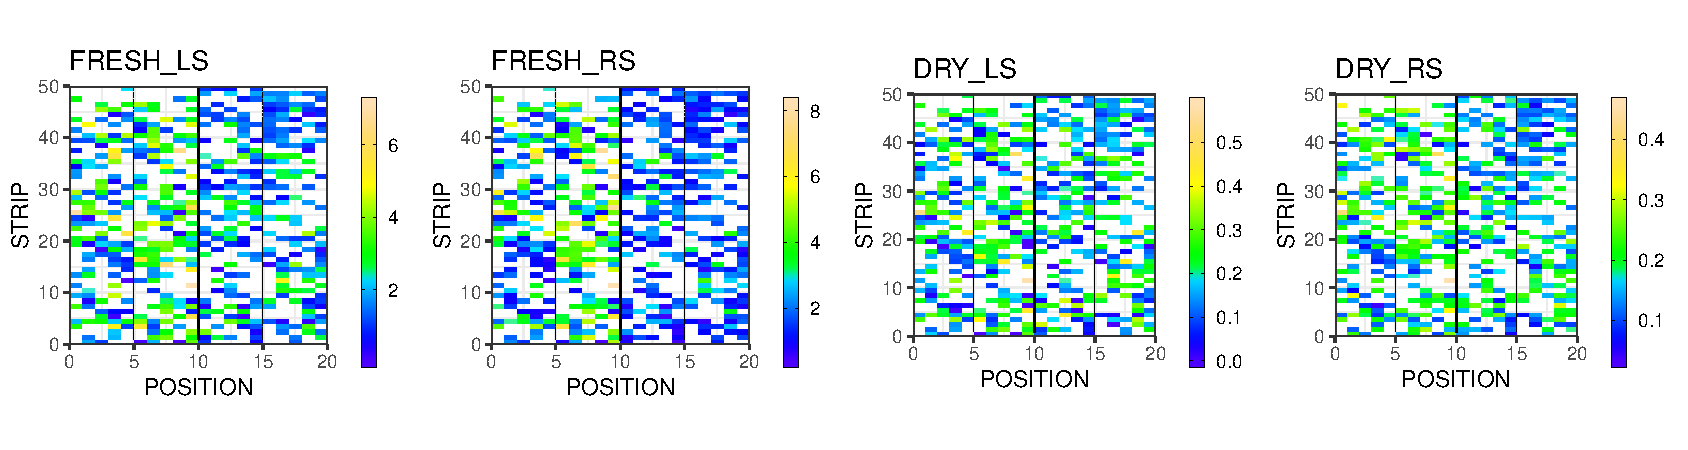
\includegraphics[width = \textwidth]{../../Figures/BSS_rawData_plot.pdf}
		\caption{Raw data}
	\end{subfigure}
	
	\begin{subfigure}[t]{\textwidth}
		\centering
		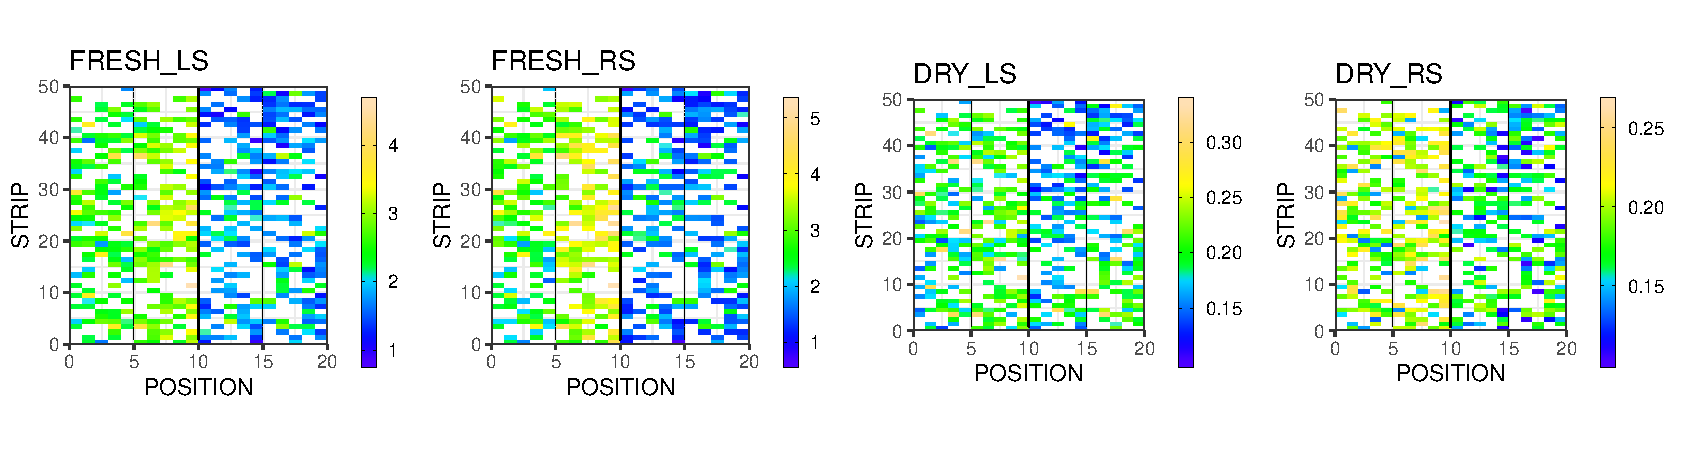
\includegraphics[width = \textwidth]{../../Figures/BSS_FittedData_plot.pdf}
		\caption{Fitted spatial trend}
	\end{subfigure}
	
	\begin{subfigure}[t]{\textwidth}
		\centering
		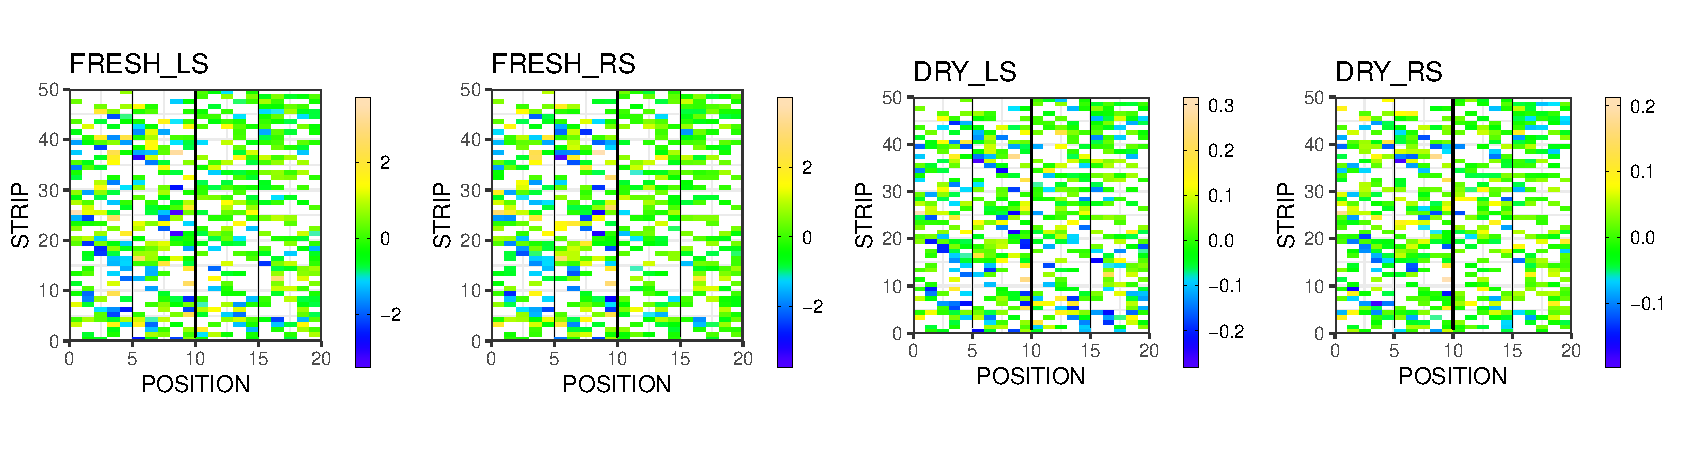
\includegraphics[width = \textwidth]{../../Figures/BSS_residuals_plot.pdf}
		\caption{Residuals' spatial plot}
	\end{subfigure}
	\caption{Raw data, fitted spatial trend and residuals' plot for each variable.}
	\label{fig:BSS_model_results}
\end{figure}

\section{Model comparison}

% Table generated by Excel2LaTeX from sheet 'Sheet1'
\begin{table}[htbp]
\rowcolors{2}{gray!25}{white}
  \centering
  \caption{Comparison of the estimated TANK fixed effect for both models.}
    \begin{tabular}{clrrrr}
    \toprule
          &       & \multicolumn{1}{l}{FRESH\_LS} & \multicolumn{1}{l}{FRESH\_RS} & \multicolumn{1}{l}{DRY\_LS} & \multicolumn{1}{l}{DRY\_RS} \\
    \midrule
    \multirow{3}[1]{*}{Tank A} & SpATS & 2,9527 & 3,7282 & 0,2164 & 0,2223 \\
          & BSS   & 2,7016 & 3,2975 & 0,2075 & 0,1959 \\
          & $\Delta$ & 0,2511 & 0,4307 & 0,0089 & 0,0264 \\
    \midrule
    \multirow{3}[1]{*}{Tank B} & SpATS & 1,3343 & 1,1445 & 0,1622 & 0,1523 \\
          & BSS   & 1,3056 & 1,1185 & 0,1660 & 0,1606 \\
          & $\Delta$ & 0,0287 & 0,0260 & 0,0038 & 0,0083 \\
    \bottomrule
    \end{tabular}%

  \label{tab:tank_effect_model_comparison}%
\end{table}%


% Table generated by Excel2LaTeX from sheet 'Sheet1'
\begin{table}[htbp]
\rowcolors{2}{gray!25}{white}
  \centering
  \caption[Comparison of both models in term of genetic variance and residual variance]{Comparison of both models in term of genetic variance and residual variance. $\Delta$ represents the absolute difference between the two variances. }
    \begin{tabular}{clrrrr}
    \toprule
          &       & \multicolumn{1}{l}{FRESH\_LS} & \multicolumn{1}{l}{FRESH\_RS} & \multicolumn{1}{l}{DRY\_LS} & \multicolumn{1}{l}{DRY\_RS} \\
    \midrule
    \multirow{3}[2]{*}{$\sigma^2_{g}$} & SpATS & 0,1709 & 0,2618 & 1,267E-03 & 6,902E-04 \\
          & BSS   & 0,1829 & 0,2644 & 1,339E-03 & 7,350E-04 \\
          & $\Delta$ & 0,0120 & 0,0026 & 7,212E-05 & 4,484E-05 \\
    \midrule
    \multirow{3}[2]{*}{$\sigma^2_{\varepsilon}$} & SpATS & 4,7073 & 5,0137 & 3,364E-02 & 1,219E-02 \\
          & BSS   & 4,5602 & 4,9245 & 3,321E-02 & 1,280E-02 \\
          & $\Delta$ & 0,1470 & 0,0892 & 4,297E-04 & 6,147E-04 \\
    \bottomrule
    \end{tabular}%

  \label{tab:sigma_model_comparison}%
\end{table}%

\begin{figure}
	\centering
	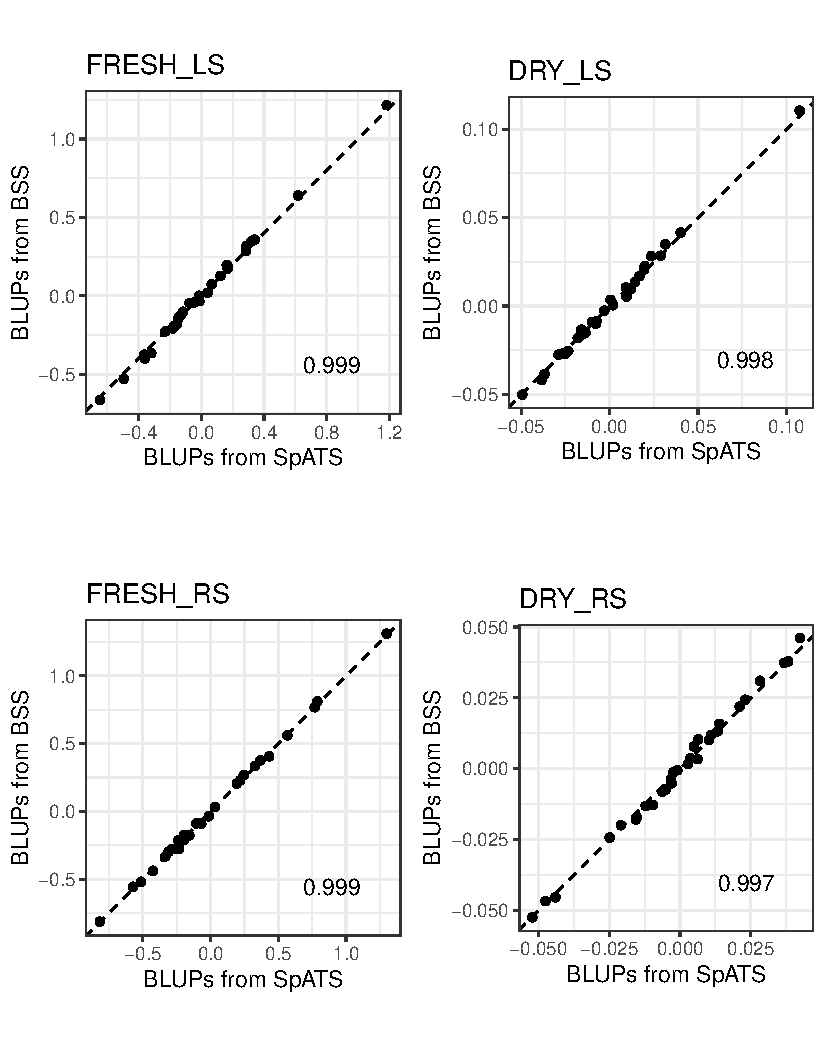
\includegraphics[width=\textwidth]{../../Figures/Genotype_Comparative_plots.pdf} 
	\caption[Comparison of the genotype BLUPs from the SpATS model and the BSS model]{Comparison of the genotype BLUPs from the SpATS model and the BSS model, with the Pearson correlation (bottom right corner of each panel).}
	\label{fig:genotype_comparison_BSS_SPATS}
\end{figure}

%\subsection{Performances}
%\subsection{Parametrization}
%\subsection{Modelling strategy}
